\documentclass[12pt]{article}
\usepackage[utf8]{inputenc}

%\newlength{\normalparindent}
%\setlength{\normalparindent}{\parindent}
%\setlength{\parindent}{\normalparindent}

\usepackage[document]{}
\usepackage{tabularx,booktabs,caption}
\usepackage{graphicx}
\usepackage[margin=1.2in]{geometry}
\usepackage{linguex}
\usepackage{natbib}
\usepackage[table, dvipsnames]{xcolor}
\usepackage{arydshln}
\usepackage{tikz-qtree}
\usepackage{amsmath}
\usepackage{amssymb}
\usepackage{bbding}
\usepackage{pifont}
\usepackage{booktabs}
\usepackage{lipsum}
\usepackage{csquotes}
\usepackage{comment}
\usepackage{endnotes}
\usepackage{xspace}
\usepackage[colorlinks=true,linkcolor=ForestGreen,citecolor=ForestGreen]{hyperref}
\usepackage{titlefoot}
\usepackage{soul}

% Colors
\definecolor{azure}{rgb}{0.94, 1.0, 1.0}
\definecolor{bluegray}{rgb}{0.4, 0.6, 0.8}

% Basic Look of the Manuscript
\newcommand{\key}[1]{\emph{#1}}
\renewcommand{\baselinestretch}{1.15}
\renewcommand{\arraystretch}{1} 
\setlength{\fboxsep}{1em}

%Macros
\newcommand{\vocab}{\mathcal{V}}
\newcommand{\mask}{\texttt{<mask>}}
\newcommand\compactdots{\hbox to 0.7em{.\hss.\hss.}}
\newcommand{\poistheta}{Pois_{\theta}}

\newcommand{\targetindex}{t}
\newcommand{\sourceindex}{s}
\newcommand{\bothindex}{\targetindex, \sourceindex}
\newcommand{\target}{$w_{\targetindex}$\xspace}
\newcommand{\targetmath}{w_{\targetindex}}
\newcommand{\Target}{$W_{\targetindex}$\xspace}
\newcommand{\Targetmath}{W_{\targetindex}}
\newcommand{\source}{$w_{\sourceindex}$\xspace}
\newcommand{\Source}{$W_{\sourceindex}$\xspace}
\newcommand{\Sourcemath}{W_{\sourceindex}}
\newcommand{\sourcemath}{w_{\sourceindex}\xspace}

\newcommand{\bw}{\mathbf{w}}
\newcommand{\maskbothmath}{\bw_{\neq \bothindex}}
\newcommand{\maskboth}{$\bw_{\neq \bothindex}$\xspace}
\newcommand{\masktargetmath}{\bw_{\notin \{\targetindex\}}}
\newcommand{\masktarget}{$\bw_{\notin \{\targetindex\}}$\xspace}
\newcommand{\context}{\texttt{c}\xspace}
\newcommand{\regression}{$R_{\sourceindex \rightarrow \targetindex}$\xspace}
\newcommand{\regressionmath}{R_{\sourceindex \rightarrow \targetindex}}

\newcommand\llh{$\mathrm{llh}$\xspace}
\newcommand{\dllmath}{\Delta_{\mathrm{llh}}}
\newcommand{\dll}{$\dllmath$\xspace}

\newcommand{\pmimath}{\operatorname{PMI}}
\newcommand{\pmi}{$\pmimath$\xspace}

\newcommand{\ppmimath}{\operatorname{PPMI}}
\newcommand{\ppmi}{$\ppmimath$\xspace}

\newcommand{\npmimath}{\operatorname{NPMI}}
\newcommand{\npmi}{$\npmimath$\xspace}

\newcommand{\kldmath}{\operatorname{KLD}}
\newcommand{\kld}{$\kldmath$\xspace}

\DeclareMathOperator*{\argmax}{\mathrm{argmax}}

\usepackage[textsize=tiny,textwidth=1in]{todonotes}
\newcommand{\note}[4][]{\todo[author=#2,color=#3,size=\scriptsize,fancyline,caption={},#1]{#4}} % default note settings, used by macros below.
\newcommand{\tiago}[2][]{\note[#1]{tiago}{cyan!40}{#2}}
\newcommand{\ryan}[2][]{\note[#1]{ryan}{violet!40}{#2}}
\newcommand{\clara}[2][]{\note[#1]{clara}{yellow!40}{#2}}
\newcommand{\ethan}[2][]{\note[#1]{ethan}{orange!40}{#2}}
\newcommand{\CR}[2][]{\note[#1]{CR note}{green!40}{#2}}
\newcommand{\Tiago}[1]{\tiago[inline]{#1}}
\newcommand{\Ryan}[1]{\ryan[inline]{#1}}
\newcommand{\response}[1]{\vspace{3pt}\hrule\vspace{3pt}\textbf{#1:}\xspace}

\title{Negative Pointwise Mutual Information Predicts Regressions during Reading}
\author{the authors}
\date{}

\begin{document}

\maketitle


\begin{abstract}
\end{abstract}

\textbf{Keywords:} 

\section{Introduction}

Reading is a learned skill that offers a unique window into the cognitive mechansisms that support real-time language comprehension. It consists of fixations, where the gaze focuses on an individual word or word-region, and saccades, where vision is surprised and gaze moves. Saccades are typically progressive (i.e. leftward moving English), however about 5\% - 20\% are regressive, going against the general flow of movement \citep{rayner1998eye}. Regressive saccades, or more simply, regressions, have played an important role in psycholinguistic theorizing, especially as clues to what types of structures people maintain in memory during real-time comprehension (e.g. \citet{jurafsky1996probabilistic}). At the same time, regressions have been analyzed from a statistical \citep{vitu2000regressive, rayner2004effects, kliegl2004length} and more recently information-theoretic \citep{bicknell2011readers, lopopolo2019dependency} perspective. 

While previous work has produced considerable insight into the role of regressions, both types of approaches---psycholinguistic and information-theoretic---are limited in their own way. There are multiple psycholinguistic theories for the causes and purpose of regressive saccades. But these tend to be qualitative in nature \citep{kennedy1987spatial, kennedy2003reader} or to make predictions for specific psycholinguistic phenomena \citep{christianson2017reread}. Because of this, it has been difficult to assess the ability of existing psycholinguistic theories to explain the wider distribution of regressions, for example over large datasets of naturalistic reading. While statistical models of reading have the potential to offer wider predictive power, the majority of these studies have focused on progressive movement through a text \citep{}. And studies that do investigate regressions have used older statistical models of language \citep{bicknell2011readers}, and focused on statistical properties of individual words rather than relationships between words. In addition, the majority of studies have focused on regressions solely in English.

The goal of the present work is to connect previous accounts of regressions with information-theoretic explanations for language processing, and to evaluate theories for regressions in a multilingual setting. Our contributions are both theoretical and experimental. Theoretically, we argue that two of the most important psycholinguistic explanations for regressions can be operationalized in terms of a widely used statistical measure of word-to-word association, Pointwise Mutual Information (PMI). Because PMI can be computed between any two words, under this interpretation both theories make generalized predictions about the distribution of regressions over  word pairs for any sentence. Experimentally, we use contemporary language models to estimate PMI over word pairs in three corpora of naturalistic reading in English, as well as for semantically controlled materials for five languages in three different language families (Italian, Spanish, German, Finnish and Turkish). We show that the negative values of PMI are strongly predictive of regressions, both within English corpora and across languages. Our results support the hypothesis that readers regress when one word causes a loss of confidence about previous word identity \cite{bicknell2011readers}. More broadly, it expands the number of language-processing behaviors that can be linked to information-theoretic principles. In the rest of this introduction we briefly introduce reading and previous theories for regressions as well as their shortcomings, motivating the present study.

\subsection{Background on Reading and Regressions}

Largely, we will discuss reading under the interpretive framework of \citet{bicknell2010rational} that views it as Bayesian inference over word identities. During each fixation, readers combine prior expectations and visual experience to update a posterior distribution over possible word identities. This distribution is maintained in memory, and can be updated subsequently. For example, a reader may change their distribution over a previous word’s identity when a new word is encountered that makes previous top candidates more or less likely. When discussing regressive saccades, or more simply regressions, we will refer to the word from which the regression originated as its source (which we denote with \source) and the word on which the regression lands as its target (\target).

We treat theories for regressions as falling into three distinct clusters. The first focuses on short within-word or between adjacent word regressions, seeking to explain them as the result of low-level ocular-motor strategies \citep{inhoff2019regressions, o1987eye, yang2001eye}. As we are largely focused on higher-level cognitive questions about how people integrate linguistic information, we will largely set these theories aside. The second cluster of theories, which we refer to as reanalysis theories, link regressions to uncertainty about previous material \citep{frazier1982making, altmann1992avoiding}. Under these theories, the source word causes the reader to lose confidence \citep{bicknell2011readers} about some interpretive choice they have made—--either a word identity or a syntactic parse—--triggering a regression to reanalyze an earlier sentence region. The last cluster, which we refer to as reactivation theories, links regressions to current word processing difficulty \citep{kennedy1987spatial, kennedy2003reader, lopopolo2019dependency}. Under these theories, regressions are used as a tool to build confidence about the current word by refocusing on (i.e. reactivating) words that support it. It’s important to stress that while each theory is distinct, they are not mutually exclusive. For example, regardless of the validity of reanalysis and reactivation theories, low-level explanations will still be required to explain the vast majority of short regressions \citep{inhoff2019regressions}. We discuss reactivation and reanalysis approaches in greater detail in Section \ref{sec:thories}.

Previous work investigating regressive saccades has reached a number of high-level conclusions about their role in reading. First, it seems that regressions are strategic. They intentionally target words or sentence regions about which the reader seeks additional information \citep{rayner1998eye} and readers can be extremely accurate at targeting specific regions of the text with regressive saccades \citep{frazier1982making, kennedy1987spatial, murray1988spatial}.\footnote{Although for a contrasting perspective which views regressions as strategic but purely as a time-buying operation, see \cite{mitchell2008accounting} and \cite{inhoff2005memory}.} Second, regressions are associated with additional information gathering, typically in the form of re-reading \citep{sturt2018processing}. For example, when reading materials are dynamically changed in between an initial fixation and a regression, subjects give answers to questions that are consistent with the changed material more than two-thirds of the time, indicating that they have re-analyzed the text \citep{booth2013function}. Finally, regressions appear to facilitate comprehension. Regression rate increases in texts that are difficult or inconsistent \citep{rayner2006eye} and suppressing regressions reduces text comprehension \citep{schotter2014don}.

Prior work also faces some serious limitations, which motivate the present study. The majority of work has tested a particular question about regressions in a controlled experimental setting. While we acknowledge the utility of such studies, it is important to balance them with experimental work that assesses the broader predictive power of each theory. And while some previous studies have attempted to do this by investigating the relationship between statistical properties of a text and regressions (e.g. \citet{vitu2000regressive, rayner2004effects, kliegl2004length, bicknell2011readers, lopopolo2019dependency}), these face a number of challenges: First, as most studies were conducted over ten years ago accurate estimates of word predictability were not available. Studies tend to either use predictability ratings from human participants \citep{rayner2004effects, kliegl2004length}, or statistical estimators that have a limited context window \citep{bicknell2011readers}.\footnote{This means that the contexts that trigger long regressions cannot be represented by these previous statistical models.} Second, previous studies have tended to focus on properties of individual words, for example looking at the unigram frequency of both a regression’s source and its target. While these properties are important, a regression is fundamentally about the relationship between two words, and thus pairwise statistical relationships like PMI may be important for understanding when and why regressions occur. Third, previous studies have tended to analyze only a single corpus at a time. Fourth, the vast majority of studies have been conducted only in English.

The final limitation concerns the type of statistical measures which previous studies have employed. Language processing involves making inferences under uncertainty \citep{kleinschmidt2015robust, bicknell2010rational} and readers may be uncertain about what they have previously read, especially if a previous word was skipped. In such cases, instead of basing the decision to regress on a previous word's realization, readers may regress based on the \textit{expectation} about its likely identity. Thus, as a second theoretical contribution, in addition to looking at actual values of PMI, we additionally investigate the role of expected PMI during regressions, where the expectation is taken over all possible realizations of the target word, \target. We argue that this measure more accurately reflects the types of decisions under uncertainty that people must make during naturalistic reading, at least vis-\`{a}-vis previous studies.

The rest of this paper will proceed as follows: In Section \ref{sec:background} we introduce the reactivation and reanalysis hypotheses for regressions in greater detail. In Section \ref{sec:info-theory} we argue that both of these can be operationalized as making predictions about the PMI between the source and target of a regression. Specifically, the reactivation hypothesis predicts that regressions should occur between words with strongly positive values of PMI (PPMI), i.e. words that are associated with each other. On the other hand, the reanalysis theory predicts that regressions should occur between words that have negative values of PMI (NPMI),  i.e. words that make each other less likely. In section \ref{sec:methods} we introduce our experimental methods: We train a Poisson model to predict the probability of a regression between pairs of words within a sentence. To compare theories, we compute the delta in held-out data's log-likelihood  under a model that includes its associated statistic (i.e. PPMI or NPMI), compared to a model that includes only the baseline statistics. If one pairwise statistic leads to higher delta log-likelihood than another, it supports its corresponding theory for regressions. Section \ref{sec:exp1} presents results from our first experiment, investigating regressions in English. Section \ref{sec:exp1} presents results from our second experiment, investigating regressions in five different languages. Our results are consistent across languages and testing environments. We find that NPMI leads to predictive power above baselines, PPMI does not. In general, expected values of NPMI have the strongest predictive power. Section \ref{sec:discussion} discusses the implications of these results, both for psycholinguistic theories as well as information-theoretic theories of language processing. Section \ref{sec:conclusions} concludes.



\section{Regressions During Reading}

In this section, we introduce previous accounts for regressions by grouping them into three theoretical clusters. We'll refer to these as \emph{low-level} theories; \emph{reanalysis}-based theories and \emph{reactivation}-based theories. Starting with \textit{low-level} approaches, these theories were developed to explain very short regressive saccades of between 1-5 characters, which constitute the majority of regressions in naturalistic reading. Low-level theories theories typically explain these regressions as corrections for longer saccades which may have over-shot their intended target \citep{inhoff2019regressions}; or as learned ocular-motor strategies in response to certain visual or motor factors \citep{o1987eye, yang2001eye}. Although interesting in their own right, we set these theories aside as they they are more related to the mechanics of ocular-motor control, rather than the integration of linguistic information, which is our focus.


%\tiago{I think this paragraph is a bit confusing imo. It doesn't really flow from the previous one, and it introduces too much stuff too fast and a bit abstractly imo. E.g., I didnt understand the "g" example. E.g.2, "We note that our sense of cueing is different from the notion of cues as linguistic representations that are content-addressable and initiate a search in memory, as is the case in the Cue-Based Retrieval approach to sentence processing \citep{lewis2013activation, mcelree2000sentence}." We introduce something here while saying our notion is different from it, from this sentence it's not super clear what "cues as linguistic representations" are, or how our view differs from it.}
\ethan{Tiago, I re-worked this paragraph a little bit. LMK what you think. The discussion of CBR is just so that certian linguists don't get confused. Also Clara, I removed your comment about mis-spellings because it was about a section of the previous paragraph that I deleted but I think that's a SUPER cool idea. My guess is that mispellings can totaly cue related words.}
For the rest of this paper, we'll focus on contrasting the reactivation and reanalysis theories for regressions. However, before turning to these directly, we introduce a unifying framework which we then use to cache out the predictions made by each theory. Specifically, we argue that both of these theories can be understood under the general neuro-psychological framework of statistical cueing. A cue is a signal, or a piece of perceptual information that reflects the state of the environment \citep{fetsch2012neural}.\footnote{We note that our sense of cueing is different from the notion of cues as linguistic representations that are content-addressable and initiate a search in memory, as is the case in the Cue-Based Retrieval approach to sentence processing \citep{lewis2013activation, mcelree2000sentence}. Rather, we mean cueing in the more general sense of statistical relatedness.} Perceptual cognition often involves the integration of multiple cues in order to form a stable percept \citep{ernst2004merging}. For example, when identifying the word ``king" one cue might be the shape of the \texttt{g}'s tail, which is integrated together with the dot on the \texttt{i}. Most relevant to our discussion is the definition from \citet{martin2016language} who defines a psycholinguistic cue as “any internal representation that signals, indicates, or is statistically related to the state of some property of the environment relevant for language processing." Thus, because g-tails and i-dots are statistically related to the word ``king" they are good cues for it.

Building on these considerations, we adopt a very simple notion of word cueing based on probability. We will think about reading as taking place in some over-all context, which we will denote with \context. (We will be more specific about this overall context in the subsequent section.) We say that a percept cues a particular word \source, if the probability of \source is higher in a context that includes the percept compared to a context without it. Because we are primarily interested in word-to-word cueing, here, we say that some word \target  cues \source with respect to some overall context if $p( \Sourcemath = \sourcemath \mid \targetmath, \context) > p( \Sourcemath = \sourcemath \mid \context)$. With this in place, we now turn to a discussion of our two main theories for regressions below.
%\tiago{Would it make sense to also measure $p( W_j = w_j \mid w_i) > p( W_j = w_j)$ as a simpler "more superficial" cueing strategy?}

\subsection{Reactivation}

Reactivation-based theories for regressions grow out of the discussion on spatial coding during reading. The spatial coding hypothesis \citep{kennedy1987spatial, kennedy1992spatial, kennedy2003reader} proposes that when readers identify words they are assigned a spatial tag, which corresponds to their position on the line. Regressions to a spatial index occur when reactivating the material associated with it can be useful for resolving processing difficulties. In particular, \citet{kennedy1987spatial} discusses cases where interpretive decisions may have to be delayed, such as when processing cataphoric pronouns like \ref{ex:cataphora}, below:

\ex. After treating him poorly, the countess apologized to the baron. \label{ex:cataphora}

In this case, a regressive saccade may be initiated between \textit{the baron} and \textit{him} because the latter's spatial location is associated with a variable that gets bound to \textit{the baron}. Crucially, the regression does not occur because the reader is confused about previous sentence material, but rather because regressing to \textit{him} reactivates a linguistic representation that facilitates current-word processing. Building on this idea, \citet{lopopolo2019dependency} suggest that regressions may be used to reactivate material that is useful for building online dependency parses. Conducting an analysis on naturalistic reading data, they show that people are more likely to regress when a word’s syntactic head or syntactic dependents are in the left context, suggesting that these are frequent targets of regressions.

One problem with these discussions is that while they assume that regressions facilitate or are useful for current operations being performed by the processor, they do not offer a single account for how one word can facilitate the processing of another. We believe that one unifying view could come from cueing. That is, people regress to previous words, or sentence indices, because the target of the regression serves as a cue for the word that triggers the regression. In Example \ref{ex:cataphora}, readers regress to \textit{him} because it serves to cue \textit{the baron}\footnote{That is, the presence of an unbound masculine pronoun in the context increases the probability that there will be a masculine animate noun later in the sentence.} and readers regress along dependency-parse edges because syntactic heads typically serve as cues to their dependents (for an information-theoretic interpretation of this see \citet{futrell2019syntactic}).

One potential challenge for the reactivation hypothesis is the following: If the reader’s goal is to identify a given word, why would they regress to another word, even if it is highly related, rather than continuing to fixate on the original word itself? One potential answer to this comes from the notion of cue integration found in the neuro-psychological literature. More robust representations of the underlying state of affairs are able to be derived when multiple cues which reflect complementary aspects of the environment are integrated together \citep{ernst2004merging}. Thus, even though regressing to a previous word may take effort, it may be the optimal strategy to achieve confidence about the current word.


\subsection{Reanalysis}

Reanalysis approaches to regressions grow out of the literature on gardenpaths, sentences which have an initial locally-plausible interpretation which is rendered impossible at a later, disambiguating, region. For example, \ref{ex:gardenpath} illustrates the well-known Main Verb / Reduced Relative (MV/RR) gardenpath effect. 

\ex. The artist painted a portrait \textbf{was impressed} by its beauty. \label{ex:gardenpath}

The sentence has an initially plausible interpretation in which \textit{painted} is a past-tense matrix verb. This becomes implausible at the disambiguating region \textit{was impressed}, in favor of a globally-plausible structural interpretation where \textit{painted} starts off a reduced relative clause. (In this case, the sentence becomes semantically equivilant to \textit{The artist who was painted a portrait was impressed by its beauty.})

Since \citet{frazier1982making} demonstrated that readers use regressions to selectively re-analyze ambiguous portions of gardenpath sentences, a number of studies have found strong links between gardenpathing and regressive saccades \citep{altmann1992avoiding}. However, as \citet{bicknell2011readers} point out, gardenpaths cannot be frequent enough to explain all regressions in naturalistic reading. They propose an alternative, but related, hypothesis in which regressions are directed towards a target not because its initial structural interpretation has become impossible (as is argued with gardenpaths) but because the reader has reduced confidence about its identity, which they dub the "falling confidence" approach. Note that the falling confidence approach can potentially explain reading behavior in gardenpath sentences. For example, in \ref{ex:gardenpath} readers may have lower confidence in the identity of \textit{painted} after they encounter \textit{was impressed}. We present both approaches together because, under both theories, regressions are triggered to reanalyze a portion of the sentence that may have been incorrectly identified previously. The crucial difference between these theories and the reactivation theories discussed above is that in the latter, the reader is assumed to have high confidence about the target of the regressive saccade, and re-fixates on it to build more confidence about the identity of the trigger. These approaches assume the opposite, namely that regressions are initiated when the reader has low confidence (or \textit{lower} confidence) about the identity of the target, and fixates on it to gain more information about its possible identity.

How do we know when one word causes a loss of confidence about a subsequent word? We adopt an intuitive notion of falling confidence based on probability. Consider two words \source, and \target, in a situation where the reader has already read \target, moved on, and is about to encounter \source. We will consider two contexts, one in which \source is known and one in which \source is not known. We will say that confidence about \target falls between the two contexts if the probability of \target is less when \source is known compared to when it is not known. That is, confidence falls when $p( \Targetmath = \targetmath \mid \sourcemath, \context) < p( \Targetmath = \targetmath \mid \context)$ (for some over-all context \context). 
One attractive feature of this formulation is that it invites a connection between falling confidence and cueing.
Specifically, it says that falling confidence is the inverse of cueing.\tiago{it's a bit weird imo to talk about a word "cueing the past". The current text talks about $w_j$ increasing prob of $w_i$, which makes this say a future word anti-cues a past word. Even if bayes rule says both probabilities (using $W_j$ to predict $w_i$ or vice versa) are the same, it's a bit weird imo.}
To make the link with the reactivation hypothesis explicit, we’ll refer to falling confidence as a case of \textbf{anti-cueing}. The reanalysis hypothesis predicts that regressions should occur between words that are anti-cues of each other.


\section{An Information-Theoretic Approach}

We make the novel claim that both previous qualitative theories for regressions embody different hypotheses about the information-theoretic relationship that should hold between the trigger and target of a regression. To simplify things, we discuss the issue in terms of \textit{lexical} causes for regressions. Following the perspective outlined in \cite{bicknell2010rational, bicknell2011readers}, we assume that reading is essentially a process of Bayesian inference about the identity of word forms and that readers maintain distributions over possible word identities as they proceed through a text. Under this perspective, regressions are used as a tool to gain more information about word identity at a particular index.

We use the following notation: For a sentence of $n$ words $w_1 \dots w_n$, \source and \target are, respectively, the source and target of a regression, where \sourceindex $>$\targetindex. They are the realizations of \Source and \Target, which are random variables with support over a vocabulary $\vocab$. The fundamental quality we are interested in is whether or not a regression occurs between \source and \target, which we model as a binary random variable, \regression. Sequences of words are indicated with bold-face script, and restrictions or holes in the sequence are indicated with subscripts. For example, the sequence of all words in a sentence excluding the trigger and target of a regression is:
%
\begin{align}
    \maskbothmath = \quad w_1 \compactdots w_{t-1},w_{t+1} \compactdots w_{s-1}, w_{s+1} \compactdots w_n \nonumber
\end{align}

Sometimes, to make the relations between terms clear, we will condition probabilities on a sequence of words with a hole, as well as an element that fills that hole. For example, $p(\sourcemath \mid \targetmath, \maskbothmath)$ gives the probability of \source conditioned on all the other words in the sentence (i.e. a context which includes \target).

To derive the predictions of each theory, we start from the notion of \textbf{surprisal}, or a word's negative log probability given its preceding context:
%
\begin{align}
    \mathrm{s}(w_i \mid \mathbf{w}_{<i}) = - \log_2 p(w_i \mid \mathbf{w}_{<i})
\end{align}

Surprisal quantifies the information content of a word. It has been shown to be implicated in numerous aspects of online sentence comprehension \citep{hale2001probabilistic, levy2008expectation, smith2013effect, wilcox2020predictive, shain2022large}, including regressions \citep{bicknell2011readers}. However, we are interested in quantifying the information content of a word in a wider variety of contexts than just its preceding words. For example, consider a situation where a reader has skipped over a word and has continued reading, potentially up until the end of the sentence. To model these sorts of contexts, we measure a word's \textbf{Cloze surprisal}, which is its negative log probability given the surrounding context:
%
\begin{align}
    \mathrm{s}_{C}(w_i \mid \mathbf{w}_{\neq i}) = - \log_2 p(w_i \mid \mathbf{w}_{\neq i})
\end{align}

Cloze surprisal is so-named for the cloze task \cite{taylor1953cloze}, in which participants have to fill in blank spots in a sentence.

\paragraph{The Reactivation Hypothesis}

What do each of the two theories say about the role of surprisal in regressions? We start first with the reactivation hypothesis, which posits that readers regress to \target because it cues (or supports) the source, \source. We adopt the intuitive notion of cuing introduced in the previous section, in which two words cue each other if knowing the identity of one makes the other more likely. This notion can be operationalized in terms of surprisal: \target cues \source if the surprisal of \source in a context where \target is known is less than in a context where \source is not known. That is, according to the reanalysis approach, the following should hold:
%
\begin{align}
    \mathrm{s_C}(\sourcemath \mid  \maskbothmath) > \mathrm{s_C}(\sourcemath \mid \targetmath, \maskbothmath)
\end{align}
The above can be re-written as the following:
\begin{align} \label{eq:pmi-frac}
    log_2 \frac{ p(\sourcemath \mid \targetmath, \maskbothmath) }{p(\sourcemath \mid \maskbothmath) } > 0
\end{align}

\noindent i.e. that the log ratio of the conditional probability of the source in a context that includes the target compared to a context that doesn't include the target should be greater than zero. The left hand side of this inequality is just the \textbf{conditional pointwise mutual information (\pmi)} between \source and \target. Pointwise mutual information is one of the most important concepts in NLP \cite{Jurafsky2000SpeechAL}. It is symmetric---that is $\pmimath(\sourcemath;\targetmath) = \pmimath(\targetmath;\sourcemath)$. It quantifies the extent to which knowing one word reduces the information content of the other word, 
%It measures how often two events co-occur, compared to what what we would expect if they were independent 
and is a well-used measure of word association. What the reactivation hypothesis predicts, then, is that regressions should occur between words when the \pmi between them is greater than zero.

But notions of cuing are not typically binary. If, instead, we assume that the strength of a cue is proportional to the ratio in Equation \ref{eq:pmi-frac}, the reactivation hypothesis predicts that not only should the \pmi between a source and target be positive, but that higher values of \pmi will correspond to stronger cues, and should be more associated with regressions. That is, the probability of a regression from \source to \target should be proportional to the positive pointwise mutual information:
%
\begin{align}
    p(&\regressionmath \mid \bw = 1) \propto \ppmimath(\sourcemath;\targetmath)
\end{align}

\noindent Where \ppmi\tiago{Can we call this $\mathrm{{PMI}}_{+}$ instead :p I think it's more readable than ppmi \response{Ethan}{ I think PPMI is standard, although I agree with your aesthetic judgement}} is the positive pointwise mutual information, i.e., $\ppmimath = \max(0, \pmimath(\triggermath;\targetmath))$.\footnote{Like PMI, PPMI is a common measure in Natural Language Processing \citep{Jurafsky2000SpeechAL}.}

\paragraph{The Reanalysis Hypothesis}

Now we turn to the reanalysis hypothesis, which posits that regressions occur between \source and \target when the presence of \source causes the reader to loose confidence about the identity of \target, or when \target is an \textit{anti-cue} of \source. Using the probablistic notion of falling confidence introduced in the previous section, but framing things in terms of surprisal values, we get that confidence falls when:
%
\begin{align}
    \mathrm{s_C}(\targetmath \mid \maskbothmath) < \mathrm{s_C}(\targetmath \mid \sourcemath, \maskbothmath)
\end{align}

\noindent Or, using the same logic as above, when:
%
\begin{align}
    \pmimath(\targetmath;\sourcemath \mid \maskbothmath) < 0
\end{align}
Following this reasoning, the reanalysis hypothesis makes the opposite prediction of the reactivation hypothesis; namely, that regressions should occur when there is a negative \pmi between two words. 

As with cuing, notions of falling confidence are not typically thought of in purely binary terms. Under our surprisal-based operationalization, the degree to which confidence falls is proportional to the value of the \pmi between \source and \target. Thus, under this framework, the reanalysis hypothesis predicts not only that the \pmi between a trigger and target should be negative, but that lower values of \pmi should be more strongly associated with regressions. That is, the probability of a regression should be proportional to negative \pmi :
%
\begin{align}
    p(&\regressionmath \mid \bw = 1) \propto \npmimath(\sourcemath;\targetmath)
\end{align}

\noindent Where $\npmimath = -min(0, \pmimath(\sourcemath;\targetmath))$ 

\paragraph{A Combined Theory:} \label{sec:combined-theory} As outlined so far, reactivation and reanalysis theories are exclusive. In the former, \pmi is associated with regressions, but only the positive range, while for the latter \pmi is only associated with regressions in the negative range. But as articulated in the literature, these theories are not necessarily in conflict. If both theories are correct, then regressions should be associated with the absolute value of the \pmi:
%
\begin{align}
    p(&\regressionmath = 1) \propto \mid \pmimath(\sourcemath;\targetmath) \mid
\end{align}

\subsection{Expectation vs. Realization} \label{sec:expectation}

So far, we have discussed regressions between two words in a context where their actual realizations are known to the reader. However, this assumption may not always hold. For example, it may be the case that the reader skipped over \target in their initial pass. In such a circumstance, readers would have to make the decision to regress not on the basis of the actual identity of \target, but rather on their expectations about \target given the context.

Thus, in addition to the operationalization presented above, we formulate an expectation-based view of each theory. Under an expectation-based view, regressions are predicted between words that have high expected value of \pmi across all possible realizations of the target variable over a vocabulary $V$:\clara{perhaps worth mentioning that its no longer a symmetric measure?}
%
\begin{align} \label{eq:expectations}
    \mathbb{E} [\pmimath(\Targetmath;\Sourcemath \mid \maskbothmath)] = \sum_{w \in V} q(w) * \pmimath(w; \sourcemath \mid \maskbothmath)
\end{align}

Where \pmi is swapped in for \ppmi or \npmi depending on the theory. We'll refer to this value as the Expected PMI or the Half-Pointwise Mutual Information. Note, that the measure is not symmetric, and that there are two possible ways to take this expectation, i.e. which distribution over \Target we choose to employ. In the first, we one could the expectation with respect to $q(\cdot) = p(\cdot \mid \maskbothmath)$ whereas in the second one could the expectation with respect to $q(\cdot) = p(\cdot \mid \sourcemath, \maskbothmath)$. The first corresponds to weighting possible values of $w$ without regard to the identity of \source (i.e. it is source-blind), while the second takes the identity of \source into account (i.e. it is source-aware). As we generally assume that readers regress only after they have read a particular source word, we believe that the source-aware expectation is more related to our behavior of interest. We note that when we plug in the vanilla \pmi into the source-aware version of Equation \ref{eq:expectations}, this becomes equivalent to the relative entropy, or KL Divergence (\kld), between \Target after and before encountering \source. (For a full discussion of the relationship to \kld, see Appendix \ref{app:kld}.)

In cases of extreme uncertainty, a reader may not only have low confidence about \target, but also about \source, too. If we were to measure expectations over both the target and the trigger of a regression, then this would give us the mutual information between the possible realizations of these two words, i.e., $\mathrm{MI}(\Targetmath;\Sourcemath \mid \maskbothmath)$. However, for our purposes here we assume that readers do know the identity of \source, and investigate only the Half-Pointwise MI outlined in Equation \ref{eq:expectations}.

\section{Experimental Methodology}

\begin{itemize}
    \item Mention that we filter words which are tokenized into two pieces because the BERT models will only give the probability of the first piece
    %\item We do not look at regressions coming from the final word in the sentence. This is due to wrap-up effects. (We did do an initial analysis that included the final word, and the results are not qualitativally different, either for Experiment 1 or Experimetn 2.)
\end{itemize}

In the following sections, we assess reactivation and reanalysis theories for regressions by asking how well NPMI and PPMI predict regressions in datasets of naturalistic reading. We estimate NPMI and PPMI from a large, pretrained language model. For each experiment, we define a set of variables which are hypothesized to impact regressions under a given theory and use them as predictors in a Poisson model trained to predict the number of regressions that occur between pairs of words. In each case, we define a baseline Poisson model, which includes various predictors that are known to have broad impact on reading behavior taken from the prior literature on reading \citep{frank2011insensitivity, smith2013effect, goodkind2018predictive, wilcox2020predictive}. In addition, we define a target Poisson model that includes baseline predictors plus our predictor of interest, e.g. PPMI or NPMI. 

Following \citet{goodkind2018predictive}, in order to assess the psycholinguistic power of our target predictors, we report the average by-word \textbf{Delta Log Likelihood ( \dll)} between baseline models and target models, where \llh is the joint log-likelihood of a dataset and \dll is the mean by-token difference in log-likelihood between the target and baseline models. Positive \dll means that models which include target predictors obtain higher likelihood on held out data over baselines; we take this as empirical support for the underlying theory associated with the predictors. In addition to asking whether the \dll is greater than zero, in order to compare different theories against each other, we  will also look at the difference in \dll between our different Poisson models. If, for example, Poisson models that include PPMI consistently obtain higher \dll than those fit with NPMI (and PPMI has a positive coefficient in the model) then we take this as additional empirical support for the reanalysis hypothesis.

\subsection{Poisson Models}

All Poisson models were fit on ten different folds of data using the \texttt{glm} function in \texttt{R} and tested on heldout data.  Predictors are normalized (i.e. $z$-scored) prior to fitting the model. For baseline predictors we included: distance between the source and the target, as well as, for both the source and target, their length (in characters);  log$_10$ frequency from \cite{speer2022wordfreq}; as well as surprisal estimated from GPT-2 \citep{radford2019language} for English or mGPT \citep{shliazhko2022mgpt} for other languages. We include four target predictors: NPMI, PPMI, as well as the expected value of the NPMI and PPMI across all possible realizations of \target, which we notate with E[NPMI] and E[PPMI].\footnote{An example call for the PPMI model: \texttt{n\_regressions $\sim$ dist + target\_len + target\_freq + target\_surp + trigger\_len + trigger\_freq + trigger\_surp + ppmi}} In addition to Poisson models that include a single target variable, we train three ensemble models---one that includes both NPMI and PPMI, one that includes both E[NPMI] and E[PPMI] and one that includes all predictors. These ensemble models instantiate the ``combined theory" we introduce at the end of Section \ref{sec:combined-theory}. Although we originally introduced the combined theory as making the prediction that regressions vary with the absolute value of the PMI, here, we include each PMI variant as a different predictors. This allows the model to find (potentially) different coefficients for the effect of PPMI and NPMI. For between model comparisons, as well as comparisons between target models and baseline models, we report the result of a pairwise permutation test.

\subsection{Datasets}

In Experiment 1, we predict human regression behavior over three dataset of naturalistic reading in English. Our datasets are: the \textbf{Provo corpus} \citep{luke2018provo} the \textbf{UCL Corpus} \citep{Frank2013ReadingTD} and the \textbf{Dundee Corpus} \citep{kennedy2003dundee}. The Provo Corpus includes data from 84 subjects reading 55 short paragraphs, or about $\sim$3,000 words of English text. The UCL Corpus contains data from 43 subjects reading 205 individual sentences totaling $\sim$ 5,00 words of English. And the Dundee Corpus contains data from 10 native English speakers reading $\sim$ 55,000 words of newspaper editorials. Overall, the Dundee Corpus contains the fewest number of participants, but much more data per participant than the other corpora.

In Experiment 2, we predict human regression behavior from a subset of the Multilingual Eye Movement Corpus (MECO) \citep{siegelman2022expanding}. MECO contains eye-tracking data on 12 simplified Wikipedia-style articles in 13 different languages. Data is collected from between 29-54 L1 speakers for each language. Articles in the corpus went through an iterative translation and back-translation process by different teams of translators to ensure that content was the same across languages. We present results from a subset of 5 languages across three different language families: German, Spanish and Italian (Ino-European), Finnish (Uralic), and Turkish (Turkic). Our languages were chosen because they have high-quality monolingual BERT-style models and are supported by mGPT, which we use to derive autoregressive surprisal estimates for baseline predictors.

\subsection{Language Models}

\begin{figure*}[t]
    \centering
    \begin{minipage}{0.95\textwidth}
    \centering
    \small
    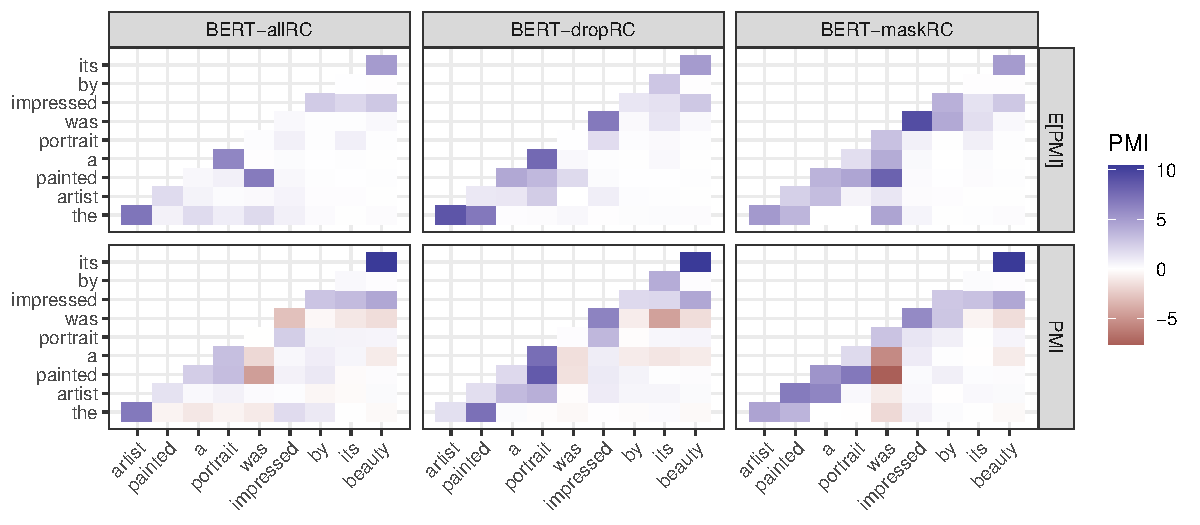
\includegraphics[width=\textwidth]{images/pmi_plotting.pdf}
    \vspace{-0.8cm}
    \caption{ \textbf{PMI estimates from BERT:} Model output is shown for a Main-Verb / Reduced-Relative Clause gardenpath sentence. The bottom row shows PMI, the top row shows expected PMI taken over all possible realizations of the target (i.e. the word on the y-axis). }
    \label{fig:pmi-example}
    \end{minipage}
\end{figure*}

We estimate the conditional PMI between \source and \target from a masked language model by taking the difference in Cloze surprisal of the \target when  \source is unmasked vs. when it is masked.\footnote{We turn PMI into NPMI and PPMI by simply zeroing out negative values (to produce PPMI) or positive values (to produce NPMI).} In Experiment 1 we use the base BERT model \cite{devlin2019bert}. In Experiment 2 we use a different BERT-style model for each language. For German we use GermanBERT \citep{deepset2019german}; for Spanish, we use BETO \citep{CaneteCFP2020}; for Finnish, we use Finnish BERT \citep{virtanen2019multilingual}; for Italian we use Italian BERT \citep{stefan_schweter_2020_4263142}; for Turkish we use BERTurk \citep{stefan_schweter_2020_3770924}. All of our models are implemented using the Huggingface Transformers library \citep{wolf2019huggingface}.

The procedure described above produces one serious discrepancy between model estimates and the information available to people when they choose whether or not to regress. Consider the sentence \textit{The dog chased the cat around the yard and barked at it}. Here, the conditional PMI between \textit{dog} and \textit{cat} is likely impacted by the presence of the subsequent word \textit{barked}. However, people read sentence incrementally and thus cannot factor future information into their representations of the context. To account for this, we derive model estimates in three settings, examples of which are given in \ref{ex:masking}.

\ex. \label{ex:masking}
\a. The \textbf{dog} chased the \textbf{cat} around the yard and barked at it {\sc [allRC]}
\b. The \textbf{dog} chased the \textbf{cat} {\sc [noRC]}
\c. The \textbf{dog} chased the \textbf{cat} \texttt{[mask]} \texttt{[mask]} \texttt{[mask]} \texttt{[mask]} \texttt{[mask]} \texttt{[mask]} \texttt{[mask]} {\sc [maskRC]}

In the \textit{allRC} setting, we give the full right context to the model. In the \textit{noRC} setting we simply truncate the sentence at the source word. And in the \textit{maskRC} setting we mask all words after the source word. In Experiment 1 we derive model estimates in all three settings. As results do not change much between settings, in Experimetn 2 we get model estimates only in the \textit{mask} setting.

To give a sense for our models' behaviors, Figure \ref{fig:pmi-example} shows the PMI and expected PMI for each of our three masking variants for a Main-Verb / Reduced Relative Clause (MVRR) gardenpath sentence. There are a couple of things to note: First, we tend to find strong positive values of PMI and E[PMI] between words that are close to each other, i.e. along the diagonal in Figure \ref{fig:pmi-example}. PMI and E[PMI] is especially strong when a noun is proceeded by a function word, such as \textit{a portrait} and \textit{its beauty}. This is because the presence of the noun severely constraints the space of possible proceeding words, making the probability of a function word much higher.\footnote{One possible concern is that because regressions most frequently occur between neighboring words, PPMI may appear to be an overly good predictor. This is why distance is included as a baseline regressor.} Second, we find negative PMI between \textit{was} and many of the other words in the sentence, with especially low PMI between \textit{was} and \textit{painted}. This is interesting, as regressions between these two sentence regions have been observed in similar human processing studies \citep{frazier1982making}. Looking at the differences between our masking setups, we find that the three are roughly comparable, although the model does seem to produce larger magnitude estimates in the \textit{dropRC} and \textit{maskRC} cases. Overall, the model behavior in Figure \ref{fig:pmi-example} provides a basic sanity-check that validates our modeling approach.

\section{Experiment 1: Regressions in English}

\begin{figure*}[t]
    \centering
    \begin{minipage}{0.95\textwidth}
    \centering
    \small
    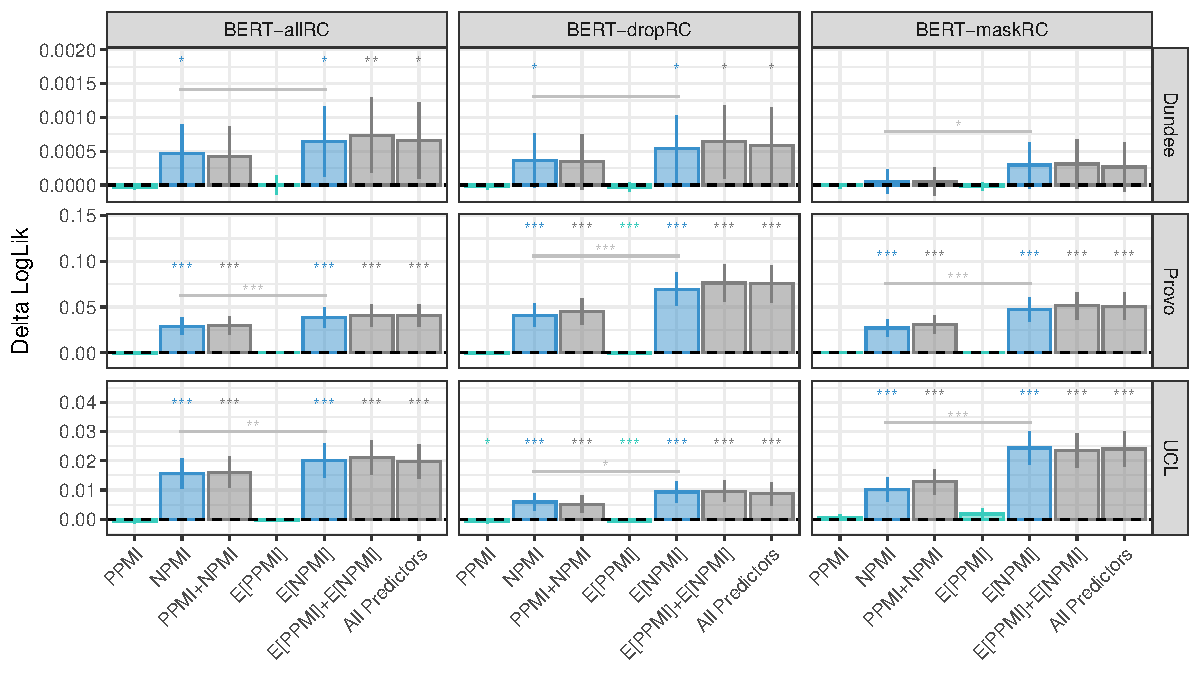
\includegraphics[width=\textwidth]{images/en_results.pdf}
    \vspace{-0.8cm}
    \caption{ \small \textbf{Results:} All models also include baseline regressors. Error bars are 95\% CIs estimated across 10-folds of data. Stars show the significance of a paired permutation test assessing whether results are different from zero. Adding (expected) Negative PMI increases \dll above baselines, indicating that these metrics are predictive of regressions in naturalistic reading. Positive PMI does not lead to increases over baselines. Overall, expected NPMI leads to the highest \dll of any (single) predictor.}
    \label{fig:exp1-results}
    \end{minipage}
\end{figure*}

\subsection{Main Results}

The results from Experiment 1 can be seen in Figure \ref{fig:exp1-results}, with models that include PPMI in red, NPMI in blue, and ensemble models in grey. The significance value from a paired permutation test testing whether the results are significantly different from zero are shown at the top. Results are consistent across masking variant and corpus tested. In every case we find that including PPMI and E[PPMI] does not lead to positive \dll and in some cases even leads to negative \dll i.e. model over-fitting (e.g. BERT-dropRC for the UCL corpus).  However, inclusion of NPMI and E[NPMI] leads to a significantly positive \dll ($p<0.001$ in all cases)\ethan{Revisit this once all the Dundee results are in!}, indicating that this statistic is predictive of regressions in naturalistic reading. Ensemble models demonstrate similar \dll as the NPMI-only models, and in some cases are even slightly worse, although this difference is not significant. Comparing realizations to expectations, E[PMI] leads to significantly higher \dll than PMI for all models over the Provo corpus ($p<0.001$) and the UCL corpus ($p<0.05$), as well as for Dundee MaskRC ($p<0.05$).\ethan{Revisit once full Dundee results are in.} Overall, these results paint a clear picture in which negative PMI is predictive of regressive saccades, and that readers are most sensitive to the expected NPI over all possible realizations of the (potential) target.

\subsection{Model Coefficients}

\begin{figure*}[t]
    \centering
    \begin{minipage}{0.95\textwidth}
    \centering
    \small
    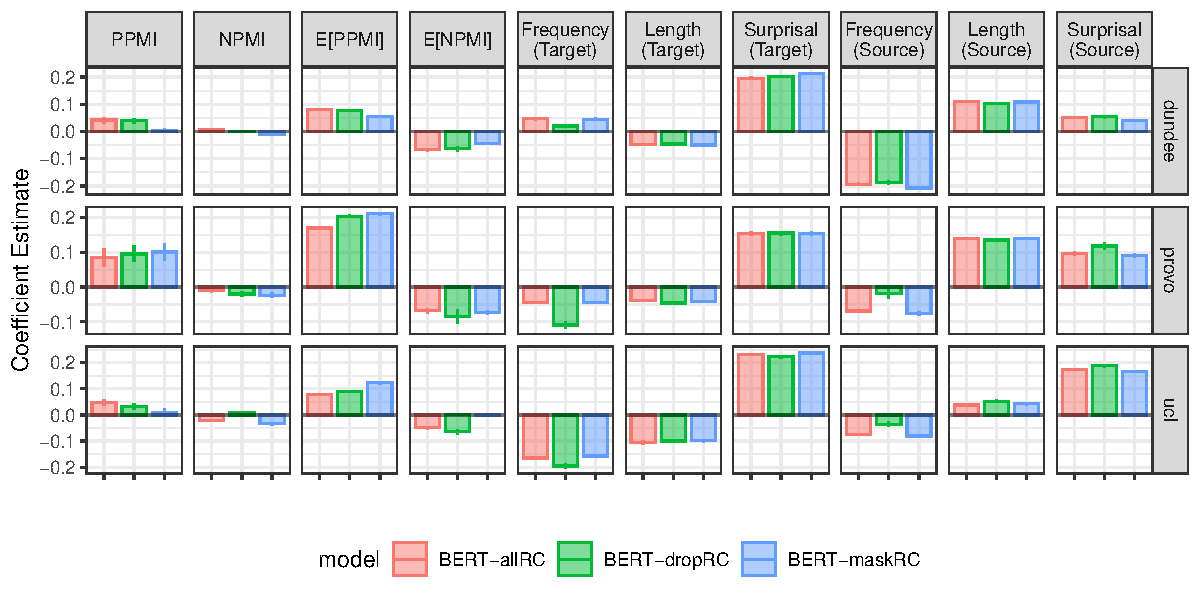
\includegraphics[width=\textwidth]{images/en_coeffs.pdf}
    \vspace{-0.8cm}
    \caption{\small \textbf{Model Coefficients:} Scaled estimates for model coefficients. Error bars are 95\% CIs across 10 folds of data. Results are similar across corpora. Distance between source and target, which has an extremely strong negative estimate is not plotted due to scale.}
    \label{fig:exp1-coeffs}
    \end{minipage}
\end{figure*}

Figure \ref{fig:exp1-coeffs} shows the coefficients of our Poisson models, for each of the relevant predictor variables. For target predictors (on the left), we show averages across all Poisson models that include the variable; for baseline predictors (on the right) we show averages across baseline models. Distance between the trigger and target is not plotted due to scale. It was found to be the strongest predictor, with negative coefficients ranging from $-3$ to $-6$, which is a full order of magnitude larger any of the other predictors. Although there is some variation, we find relatively strong consistency in terms of coefficient sign and magnitude across datasets and models. Starting first with our baseline variables, we find a relatively large positive effect of surprisal for both source and target words, indicating that as the predictability of both words goes down, the likelihood of a regression between them increases. For frequency, we find a negative effect for both source and target words, indicating that regressions are more likely to occur between low frequency words. This effect tends to be a little stronger for the source word, especially in the Dundee and UCL corpora. Finally, we find a mixed result for word length: In the Provo and Dundee corpora, there is a negative effect of target length, however this is slightly positive in the UCL corpus. We find a positive coefficient for source-word length across all corpora. These results suggest that as the source word increases in length regressions are more likely to be initiated, but regressions do not necessarily target longer words.

Turning to the target predictors, as expected, we find positive coefficients for PPMI and E[PPMI], and negative coefficients for NPMI and E[NPMI] (except for the BERT-maskRC in the UCL corpus, where the effect is slightly positive.) Effect sizes for expectations tend to be larger than those for the realization values (i.e. PPMI and NPMI) themselves, which is consistent with the main results that expectations lead to higher \dll. Interestingly, we find that logistic models fit larger estimates for PPMI and E[PMI], even though PPMI was not found to impact \dll.

\subsection{Discussion of Results}

The results of this experiment suggest that regressions occur because readers are sensitive to how the current word changes the respective probabilities of previous words. If a current word makes a previous word less likely, i.e. higher surprisal, then a regression is likely to occur between them. Even more interestingly, though, the strong results for E[NPMI] suggest that readers are not only sensitive to the relative likelihood of the actual words they have encountered, but additionally to their alternative possible realizations. When a good number of the likely realizations are made more surprising, then regressions are even more likely to occur. Finally, these results do not support the combined theory for regressions; ensemble models that included both PPMI and NPMI do not lead to higher \dll than models that include solely NPMI or E[NPMI]. This suggests that it is purely falling confidence in previous material that drives regressions during reading.

In addition to this novel PMI-based statistics, this experiment used a number of baseline predictors that have been previously investigated in the literature, largely confirming previous findings. We place our discussion of these results here, rather than in the general discussion, because previous work has focused on English. Starting with cases where the literature agrees, prior work has found that target words tend to be low predictability \citep{rayner2004effects, kliegl2004length} or higher surprisal \citep{bicknell2011readers}, which is in line with our positive effect of target surprisal. Prior work is mixed, however, when it comes to the surprisal of the source: \citet{bicknell2011readers} find a negative effect of predictability (i.e. a \textit{positive} effect of surprisal) but \cite{lopopolo2019dependency} find a negative effect. Although the magnitude of the surprisal effect is greater for targets than sources, we do find a significantly positive effect of source-word surprisal for all corpora and masking types which supports the results form \citet{bicknell2011readers}.

Prior studies are mixed when it comes to frequency and length: Focusing first on target words, two studies have found no effect of target frequency \citep{rayner2004effects, kliegl2004length}, while another has found a positive effect \citep{bicknell2011readers}. Ours is the first study to report a negative effect. For word length, some studies found that regressions target short words \citep{kliegl2004length} and other that they target longer word \citep{vitu2000regressive, bicknell2011readers}. The results for this study support a negative effect for target word length, although note that effects were (slightly) positive for the UCL corpus. Effects of source words on regressions are less common in the literature. Our results support the negative effect found previously by \cite{lopopolo2019dependency}\footnote{Note that \citet{bicknell2011readers} actually find a positive effect for source word frequency, however the result is not significant.} Overall, where previous studies agree our results are in line with previous work (e.g. on the positive effect of target word surprisal and the negative effect for target word length).

In sum, these results suggest that regressions are likely to occur when the source word is difficult to process (it is high surprisal, long and low frequency), and the target it somewhat difficult to process (it is higher surprisal, although not necessarily long or very low frequency). 


\section{Experiment 2: Crosslinguistic Study }

\begin{figure*}[t]
    \centering
    \begin{minipage}{0.95\textwidth}
    \centering
    \small
    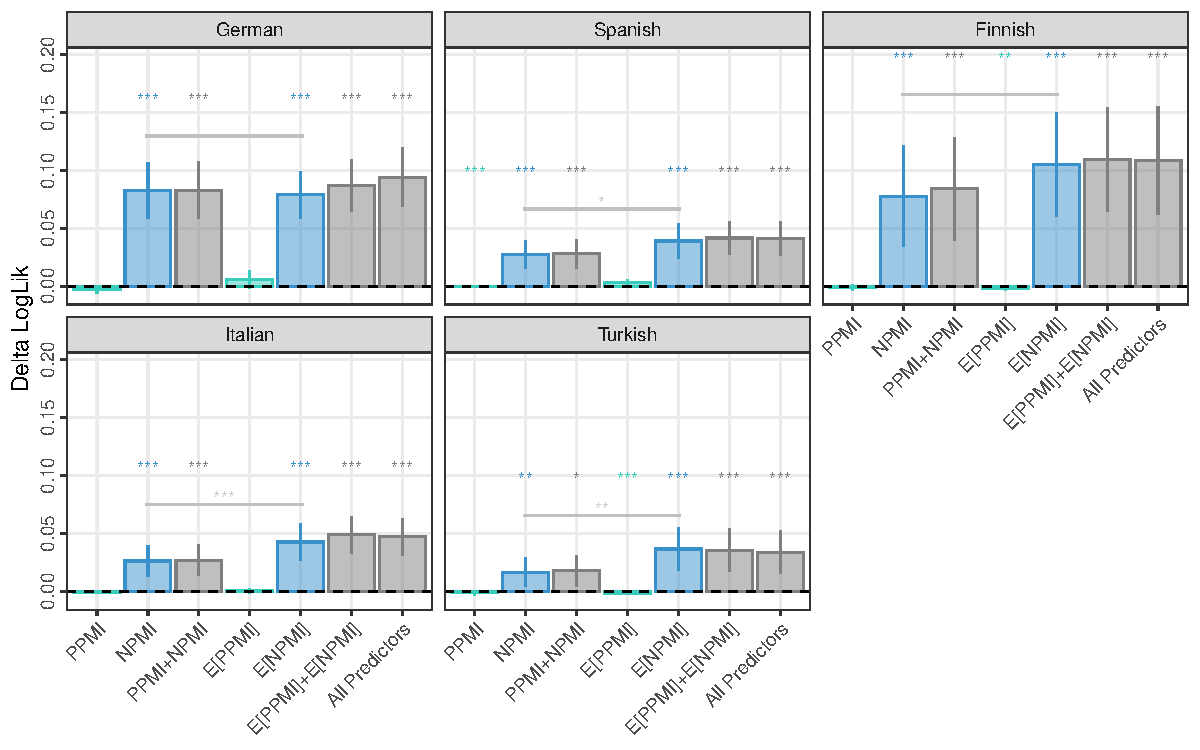
\includegraphics[width=\textwidth]{images/meco_results.pdf}
    \vspace{-0.8cm}
    \caption{ \small \textbf{Results:} All models also include baseline regressors. Error bars are 95\% CIs estimated across 10-folds of data. Stars show the significance of a paired permutation test assessing whether results are different from zero. Adding (expected) Negative PMI increases \dll above baselines, indicating that these metrics are predictive of regressions in naturalistic reading. Positive PMI does not lead to increases over baselines.}
    \label{fig:exp2-results}
    \end{minipage}
\end{figure*}

In this study, we ask whether the results obtained for English hold up in a broader sample of languages. We investigate German, Spanish, Finnish, Italian and Turkish, which represent three different language families: Indo-European, Uralic and Turkic. For this study we use the {\sc maskRC} setup from the previous study. This was done because it intuitively is the closest to human language processing: People are not  aware of word identity in their right context\footnote{They do obtain some, albeit very little, information from parafoveal vision \citep{schotter-etal:2012-parafoveal}}, but they are aware that the sentence continues, a situation which is better encapsulated with the {\sc maskRC} setting over the {\sc noRC} setting or the {\sc allRC} setting.

\subsection{Main Results}

The main results from this study can be seen in Figure \ref{fig:exp2-results}. The presentational paradigm is the same as from the first study, except that the different languages are shown in the x-facets. The results are extremely consistent across languages and support the results from the previous experiment. For all languages tested, PPMI and E[PPMI] either lead to no gain in \dll, or to negative \dll, indicating that they lead to overifitting in the Poisson models. NPMI, on the other hand, leads to significantly positive \dll in every language ($p<0.001$) except Finnish. And E[NPMI] leads to higher \dll in every language tested ($p<0.001$). Ensemble models have a similar \dll to models with just NPMI or E[NPMI], except for Finnish and Italian, where the inclusion of E[PPMI] in models with all predictors leads to over-fitting. As with Experiment 1, E[NPMI] tends to lead to higher \dll than bare NPMI. This difference is significant in all languages ($p<0.001$), except in German it is significant in the opposite direction; that is, NPMI leads to higher \dll than E[NPMI].

\subsection{Model Coefficients}

\begin{figure*}[t]
    \centering
    \begin{minipage}{0.95\textwidth}
    \centering
    \small
    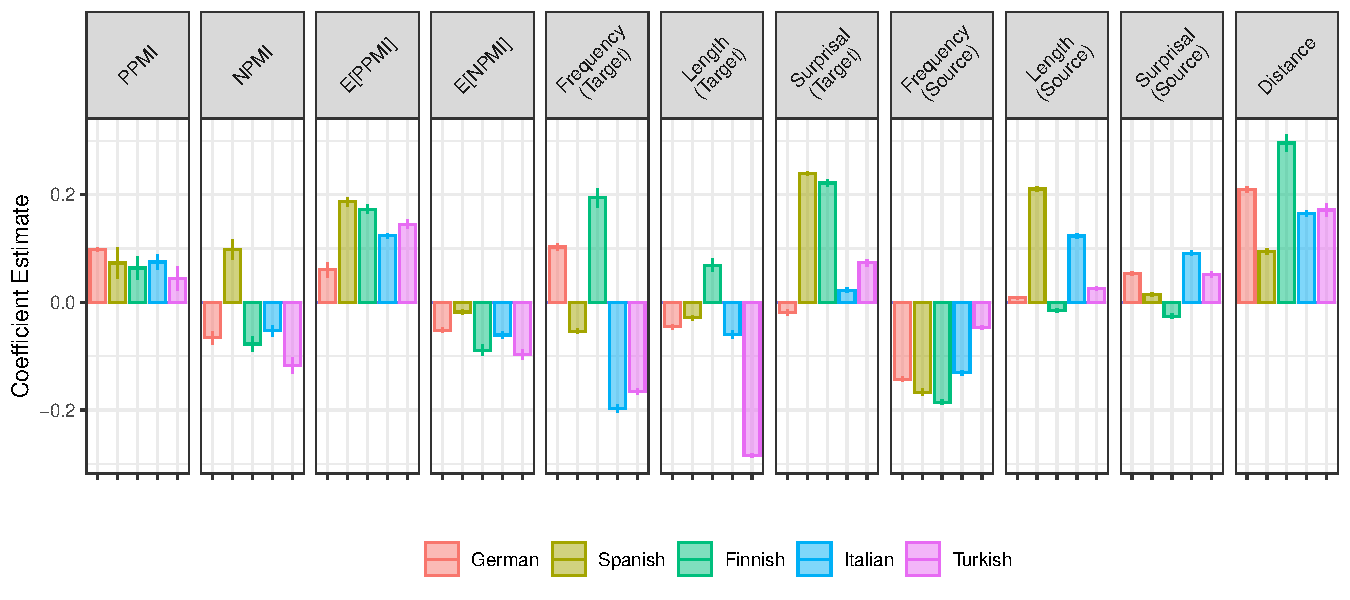
\includegraphics[width=\textwidth]{images/meco_coeffs.pdf}
    \vspace{-0.8cm}
    \caption{ \small \textbf{Model Coefficients:} Scaled estimates for model coefficients. Error bars are 95\% CIs across 10 folds of data. Results are similar across corpora. Distance between source and target, which has an extremely strong negative estimate is not plotted due to scale.}
    \label{fig:exp2-coeffs}
    \end{minipage}
\end{figure*}

The coefficients of our Poisson models are shown in Figure \ref{fig:exp2-coeffs}. Although results are largely in line with the results from Experiment 1, we do observe some variance between languages. Focusing first on the baseline predictors, the biggest difference between this experiment and Experiment 1 is that, here, we observe a positive effect of distance. This indicates that regressions were more likely to occur between words that were further away from each other, within a sentence. In line with Experiment 1, we find positive effects of surprisal for both the source and the target (in 4/5 languages for each) as well as negative effects of source word frequency in every language. Effect directions are mixed for target word frequency, as well as for word length, which is not necessarily surprising given the mixed findings in the prior literature testing these variables. Turning to our target predictors, we find positive effects for E[PMI] and PMI, and negative effects for E[NPMI] and NPI (except for Spanish, where the effect is positive).

\subsection{Discussion of Results}

We believe that the crosslinguistic consistency evident in Figure \ref{fig:exp2-results} is rather striking. It provides compelling evidence that the same information-theoretic principles are at play during language processing in multiple languages, suggesting that readers maintain distributions over prior words forms and regress when new material causes previous words to become less likely. There are, however, some intriguing differences between these results and those from Experiment 1. First, we observe that in German, the NPMI between the source and the actual target, \target, is a better predictor of regressions than the expected PMI over potential targets. In Experiment 1, and for other languages in Experiment 2, we observed larger \dll for E[NPMI]. So what's going on with German? We hypothesize that these results would be consistent with a strategy in which German readers spend more time identifying and committing to the actual word \target, and are thus more sensitive to  changes in its relative likelihood (at least vis \`{a} vis readers in other languages). There are a few pieces of evidence supporting this hypothesis: German readers were found to have a low skip-rate and, more tellingly, a very low overall reading-rate in the MECO dataset, suggesting that their reading strategy may involve a more methodical pass over the text. That being said, the reading rate was actually slower for Finnish readers. Although we believe that this `early commitment' theory is a promising hypothesis, further investigation of German reading data is needed.

The second question we address concerns the positive effect of distance observed in Experiment 2. In Experiment 1, we found an extremely strong negative effect of distance---that is, there were far more regressions between adjacent words than distal words. Why, then, do we observe a stable, positive effect across languages for the MECO data? We hypothesized that this has to do with \textit{wrap-up effects}. Wrap-up effects are regressions or longer reading times that occur at the ends of sentences and are thought to be caused by the reader consolidating the information contained in the sentence before moving on to the next one \textbf{(citations)}. \textbf{Because the MECO dataset includes longer texts, participants are more likely to wrap-up at the end of each sentence, and glance to previous portions of the sentence. Supporting this hypothesis, we found that regressions originating at the ends of sentences tended to be longer than those that did not (numbers).} In order to test this hypothesis, we re-ran the analysis of Experiment 2 excluding all regressions that originated from sentence final words. After this exclusion, we observed a strong negative effect of distance, confirming our hypothesis. We note that, after this exclusion, the over-all pattern of main results did not change; Models with NPMI and E[NPMI] still showed positive \dll, whereas models with PPMI and E[PPMI] did not.\footnote{We also ran this analysis on the English only data from Experiment 1 with similar results. Exclusion of sentence-final regressions does not change the qualitative picture of results, although the smaller amount of data does mean that error estimates are larger, especially for the Dundee dataset.}

\section{General Discussion}

\begin{itemize}
    \item Discussion of expectation as quite remarkable, given that in an expectation, the negative quantities will always have a lower value than the positive quantities. Thus, even though the positive values are, in some sense, a stronger signal, people are still sensitive to the negative values.
    \item Discussion of our "expectation" measure. We compute the expectation over all possible realizations of the vocabulary but this may be intractable during language processing. Maybe the reader is actually sensitive to some weighted expectation.
    \item Negative Pointwise Mutual Information is something that has been previously critiqued in the Natural Language Processing literature, for two reasons. Because of these reasons, PMI is typically replaced with PPMI (citations). At a theoretical level, when two words have a negative PMI, it means that they occur together less than would be expected by chance. Explain why people don’t like this. However, our discussion of PMI as essentially about surprisal values offers a different, and useful, interpretation. Under our interpretation a negative PMI indicates the extent to which the presence of one word increases the surprisal (i.e. information content) of the other, given some overall context. The second reason people tend to avoid NPMI is that you need a large corpus of text to estimate it. Example from Jurafsky. Modern transformers, which are fit on large amounts of data alleviate this problem. Discuss the dataset size of BERT and mBERT.
    \item Discuss this in the context of the anticipation paper. Can we explain forward and backwards movement through a text purely on information-theoretic terms?
    \item Discussion of these results in the context of \cite{futrell2019information}
\end{itemize}


\section{Conclusion}


\bibliographystyle{apalike}
\bibliography{everything}


\appendix


\section{Relationship between Expected PMI and KLD} \label{app:kld}

In Section \ref{sec:expectation} we suggest that readers may be sensitive to the expected value of \pmi between a known source and unknown target. We mention that there are two possible ways to take this expectation---source-aware and source-blind. In this appendix we connect each of these expectations to a well-known distance metric, the KL Divergence, or \kld. Specifically, we connect these two expectations to \kld between the probability distribution over possible targets when the source is known (i.e. $\Targetmath \mid \source, \maskbothmath$) and the distribution over possible targets when the trigger is not known (i.e. $\Targetmath \mid \maskbothmath$).

\paragraph{Trigger-Aware Expectation} We begin with the source-aware expectation. By substituting the equation for PMI, we see that the expectation is equivalent to the \kld of \Target after vs. before encountering \source:
%
\begin{align}
    \mathbb{E}&[\pmimath(\Targetmath;\sourcemath \mid \maskbothmath)] \nonumber \\
    &= \sum_{w \in V} p(\Targetmath = w \mid \sourcemath, \maskbothmath) * \pmimath(\Targetmath = w; \Sourcemath = \sourcemath \mid \maskbothmath) \\
    &= \sum_{w \in V} p(\Targetmath = w \mid \sourcemath, \maskbothmath) * log_2 \frac{p(\Targetmath = w \mid \sourcemath, \maskbothmath)}{p(\Targetmath = w \mid \maskbothmath)} \\
    &= \kldmath(\Targetmath \mid \sourcemath, \maskbothmath \mid \mid \Targetmath \mid \maskbothmath )
\end{align}

\paragraph{Trigger-Blind Expectation} We show that the negative value of the trigger blind expectation is equivilant to the \kld of \Target before vs. after encountering \trigger:
%
\begin{align}
    - \mathbb{E}&[\pmimath(\Targetmath;\sourcemath \mid \maskbothmath)] \nonumber \\
    &= - \sum_{w \in V} p(\Targetmath = w \mid \maskbothmath) * \pmimath(\Targetmath = w; \Sourcemath = \sourcemath \mid \maskbothmath) \\
    &= - \sum_{w \in V} p(\Targetmath = w \mid \maskbothmath) * log_2 \frac{p(\Targetmath = w \mid \sourcemath, \maskbothmath)}{p(\Targetmath = w \mid \maskbothmath)} \\
    &= \sum_{w \in V} p(\Targetmath = w \mid \maskbothmath) * log_2 \frac{p(\Targetmath = w \mid \maskbothmath)}{p(\Targetmath = w \mid \sourcemath, \maskbothmath)} \\
    &= \kldmath(\Targetmath \mid \maskbothmath \mid \mid \Targetmath \mid \sourcemath, \maskbothmath )
\end{align}


\end{document}